\begin{figure}[H]
\centering
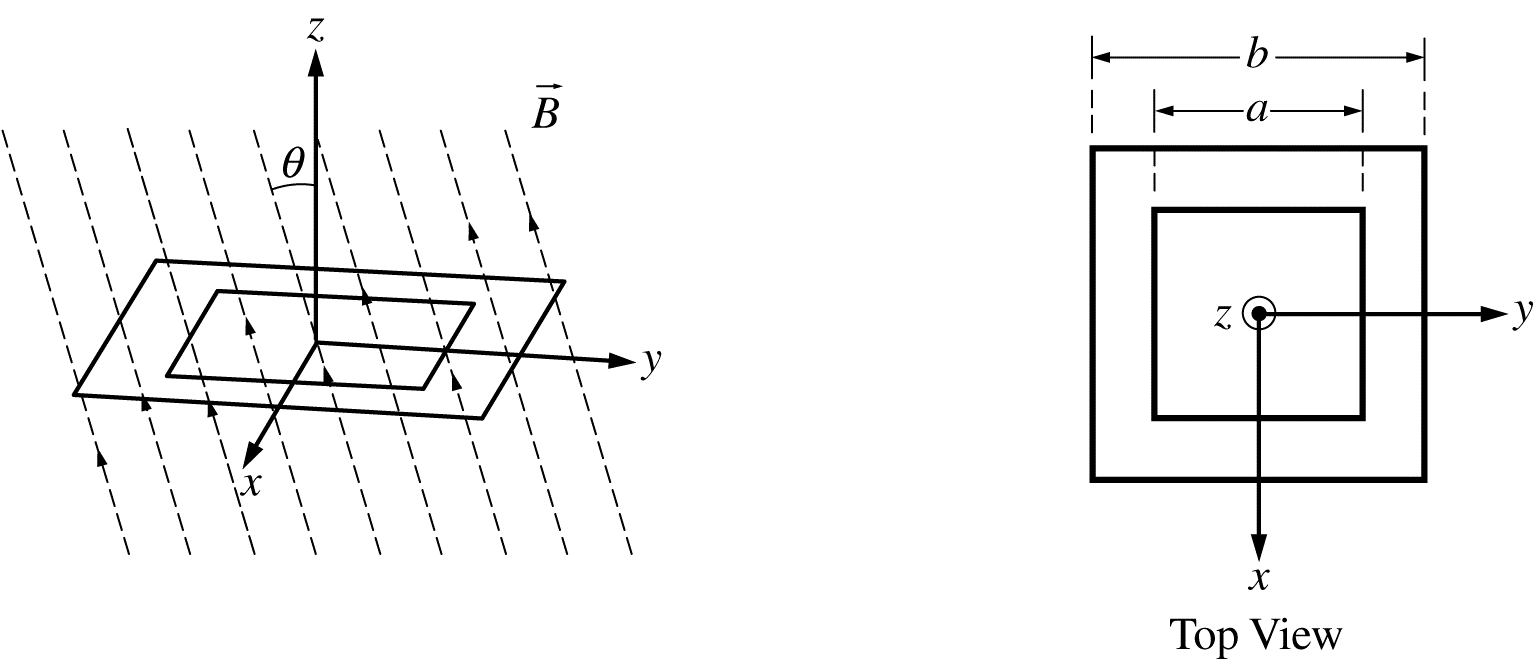
\includegraphics[scale=0.25]{images/img-014-040.png}
\end{figure}

% Multiple Choice Question 33
\begin{questions}\setcounter{question}{32}\question
Two square loops of thin metal wire are positioned on the horizontal $x y$-plane in a magnetic field $\vec{B}$ that is directed upward through the loops at an angle $\theta$ with the vertical z-axis, as shown in the figure above. The small loop has side length $a$. The large loop has side length $b$. The magnetic flux in the space between the loops is

\begin{oneparchoices}
\choice $B\left(b^{2}-a^{2}\right) \sin \theta$
\choice $B\left(b^{2}-a^{2}\right) \cos \theta$
\choice $B(b-a)^{2} \cos \theta$
\choice $B a^{2} \sin \theta$
\choice $B b^{2} \sin \theta$
\end{oneparchoices}\end{questions}

